\section{Overview of the pseudonymisation}

\begin{figure}
\centering
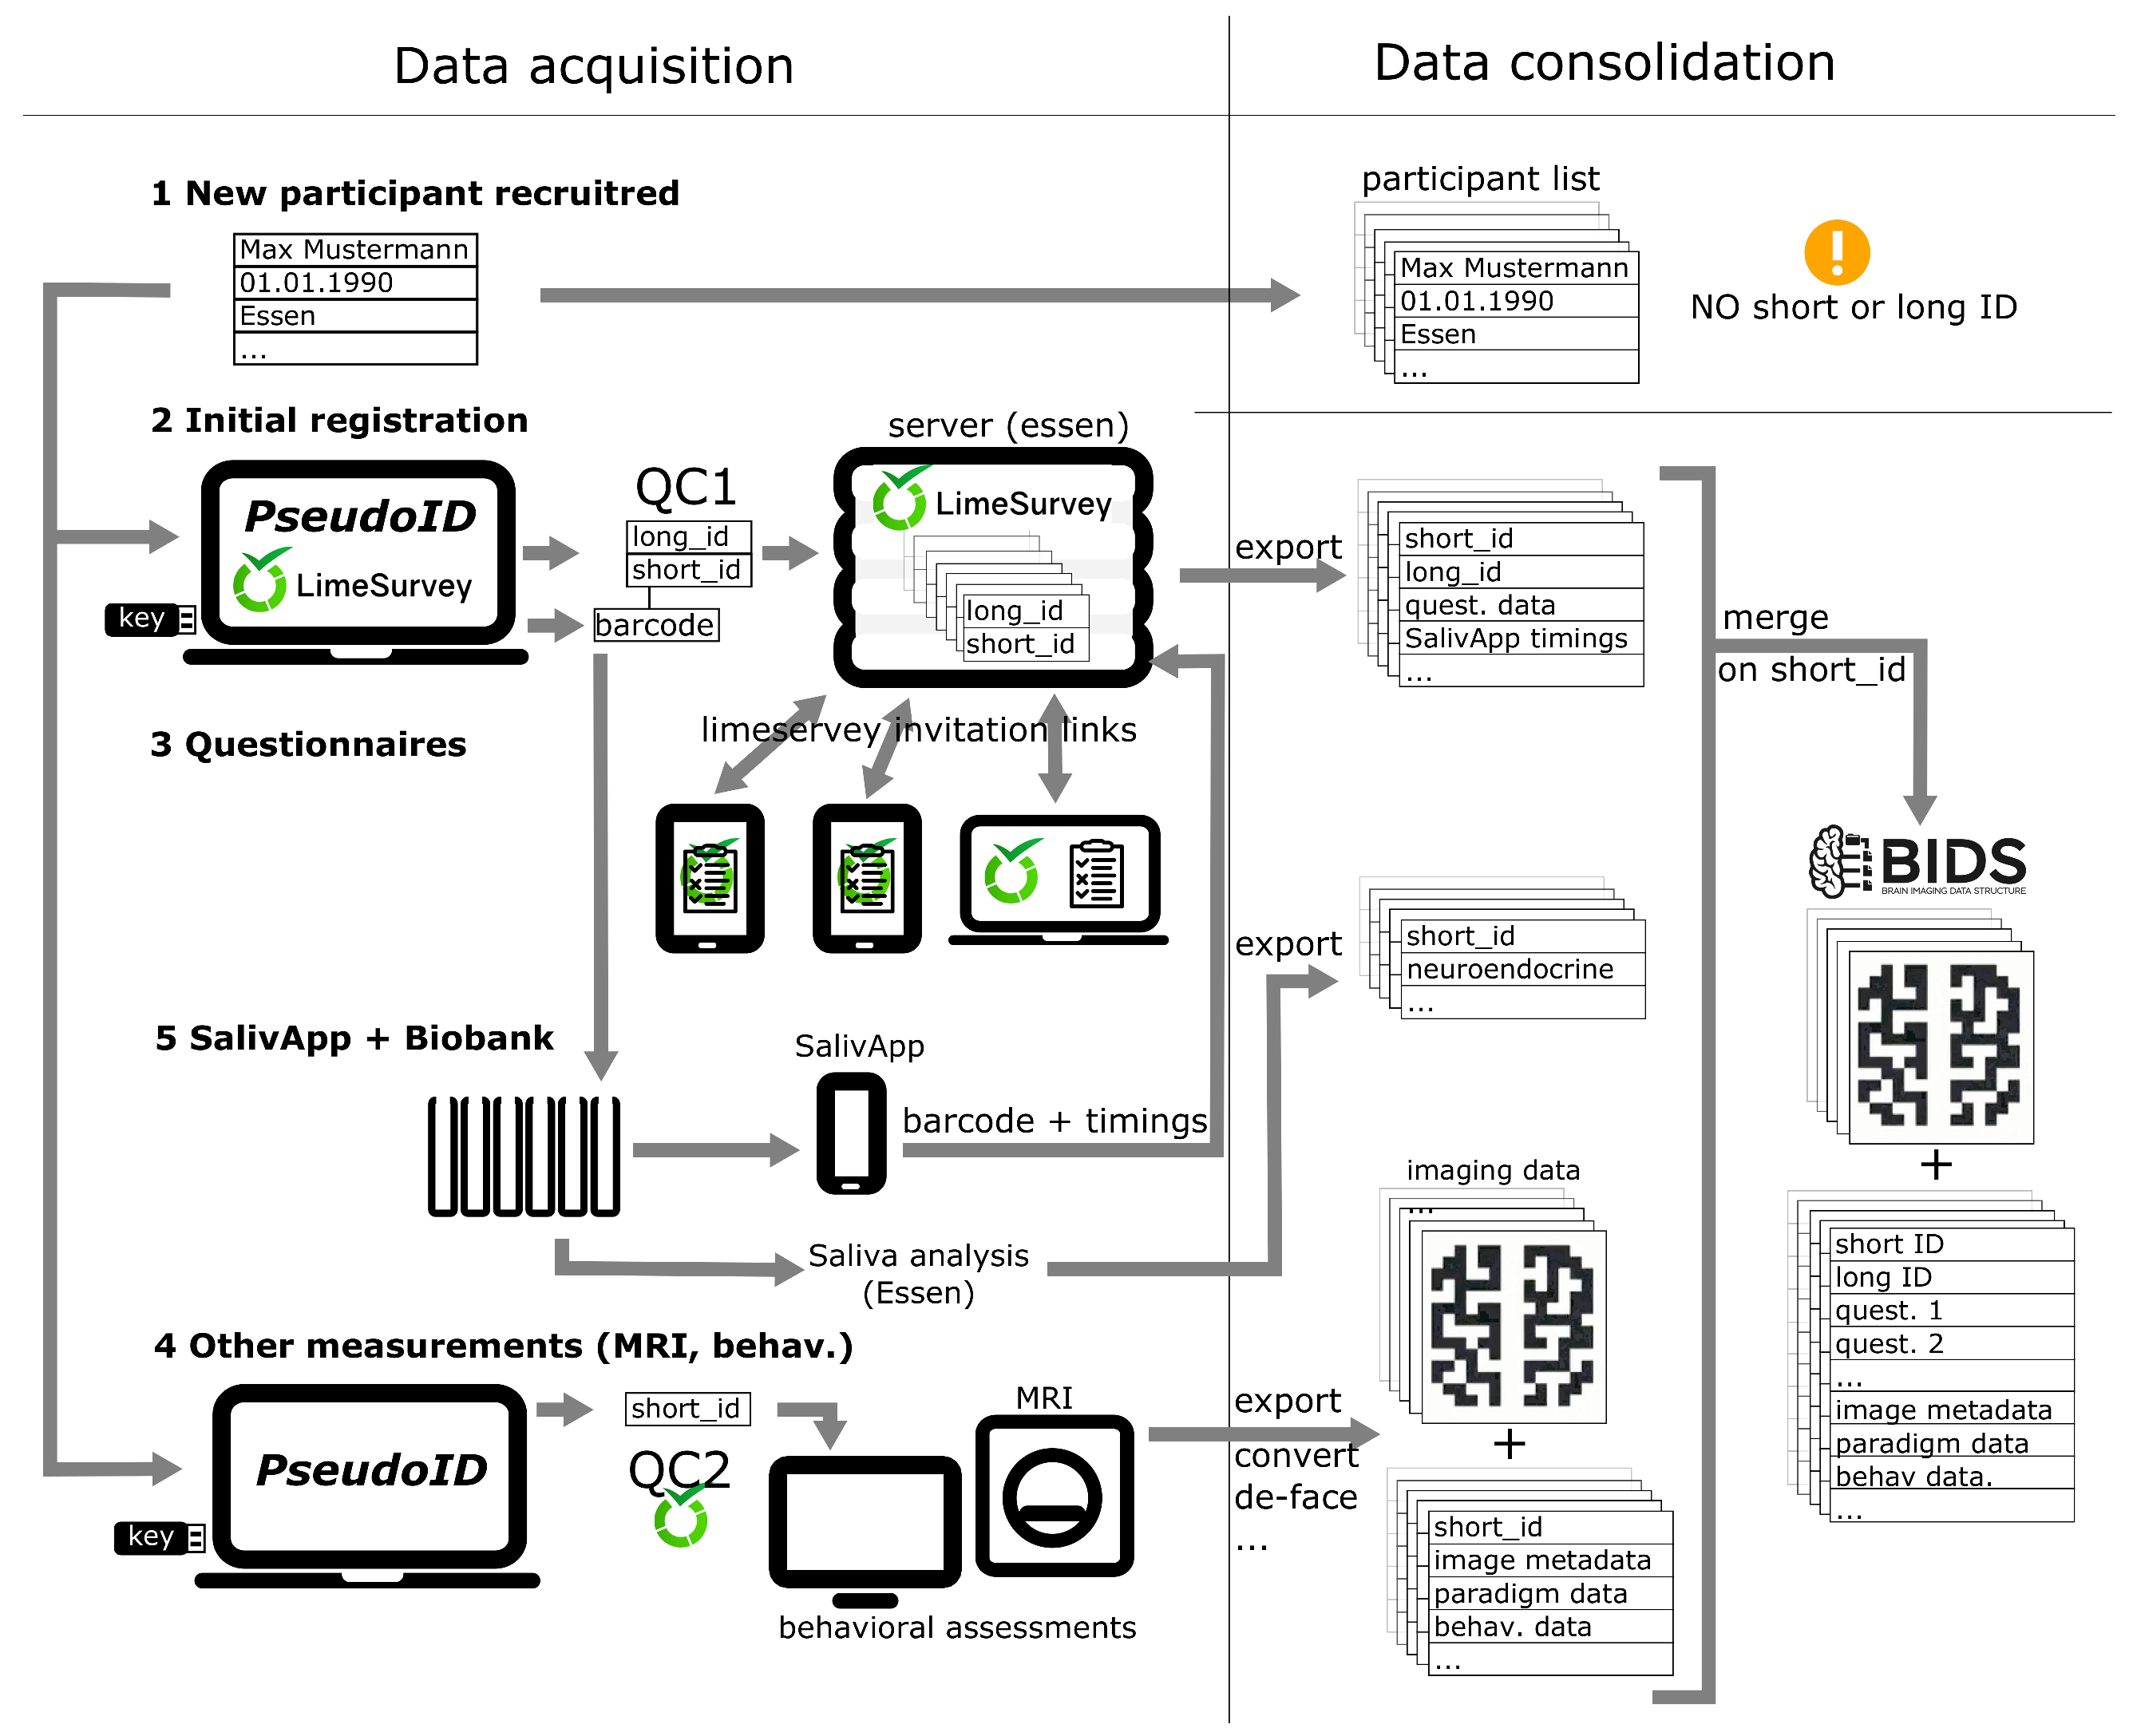
\includegraphics[width=1.0\textwidth]{docs/fig/overview_v2.eps}
\end{figure}

\begin{figure}
\centering
\subfigure{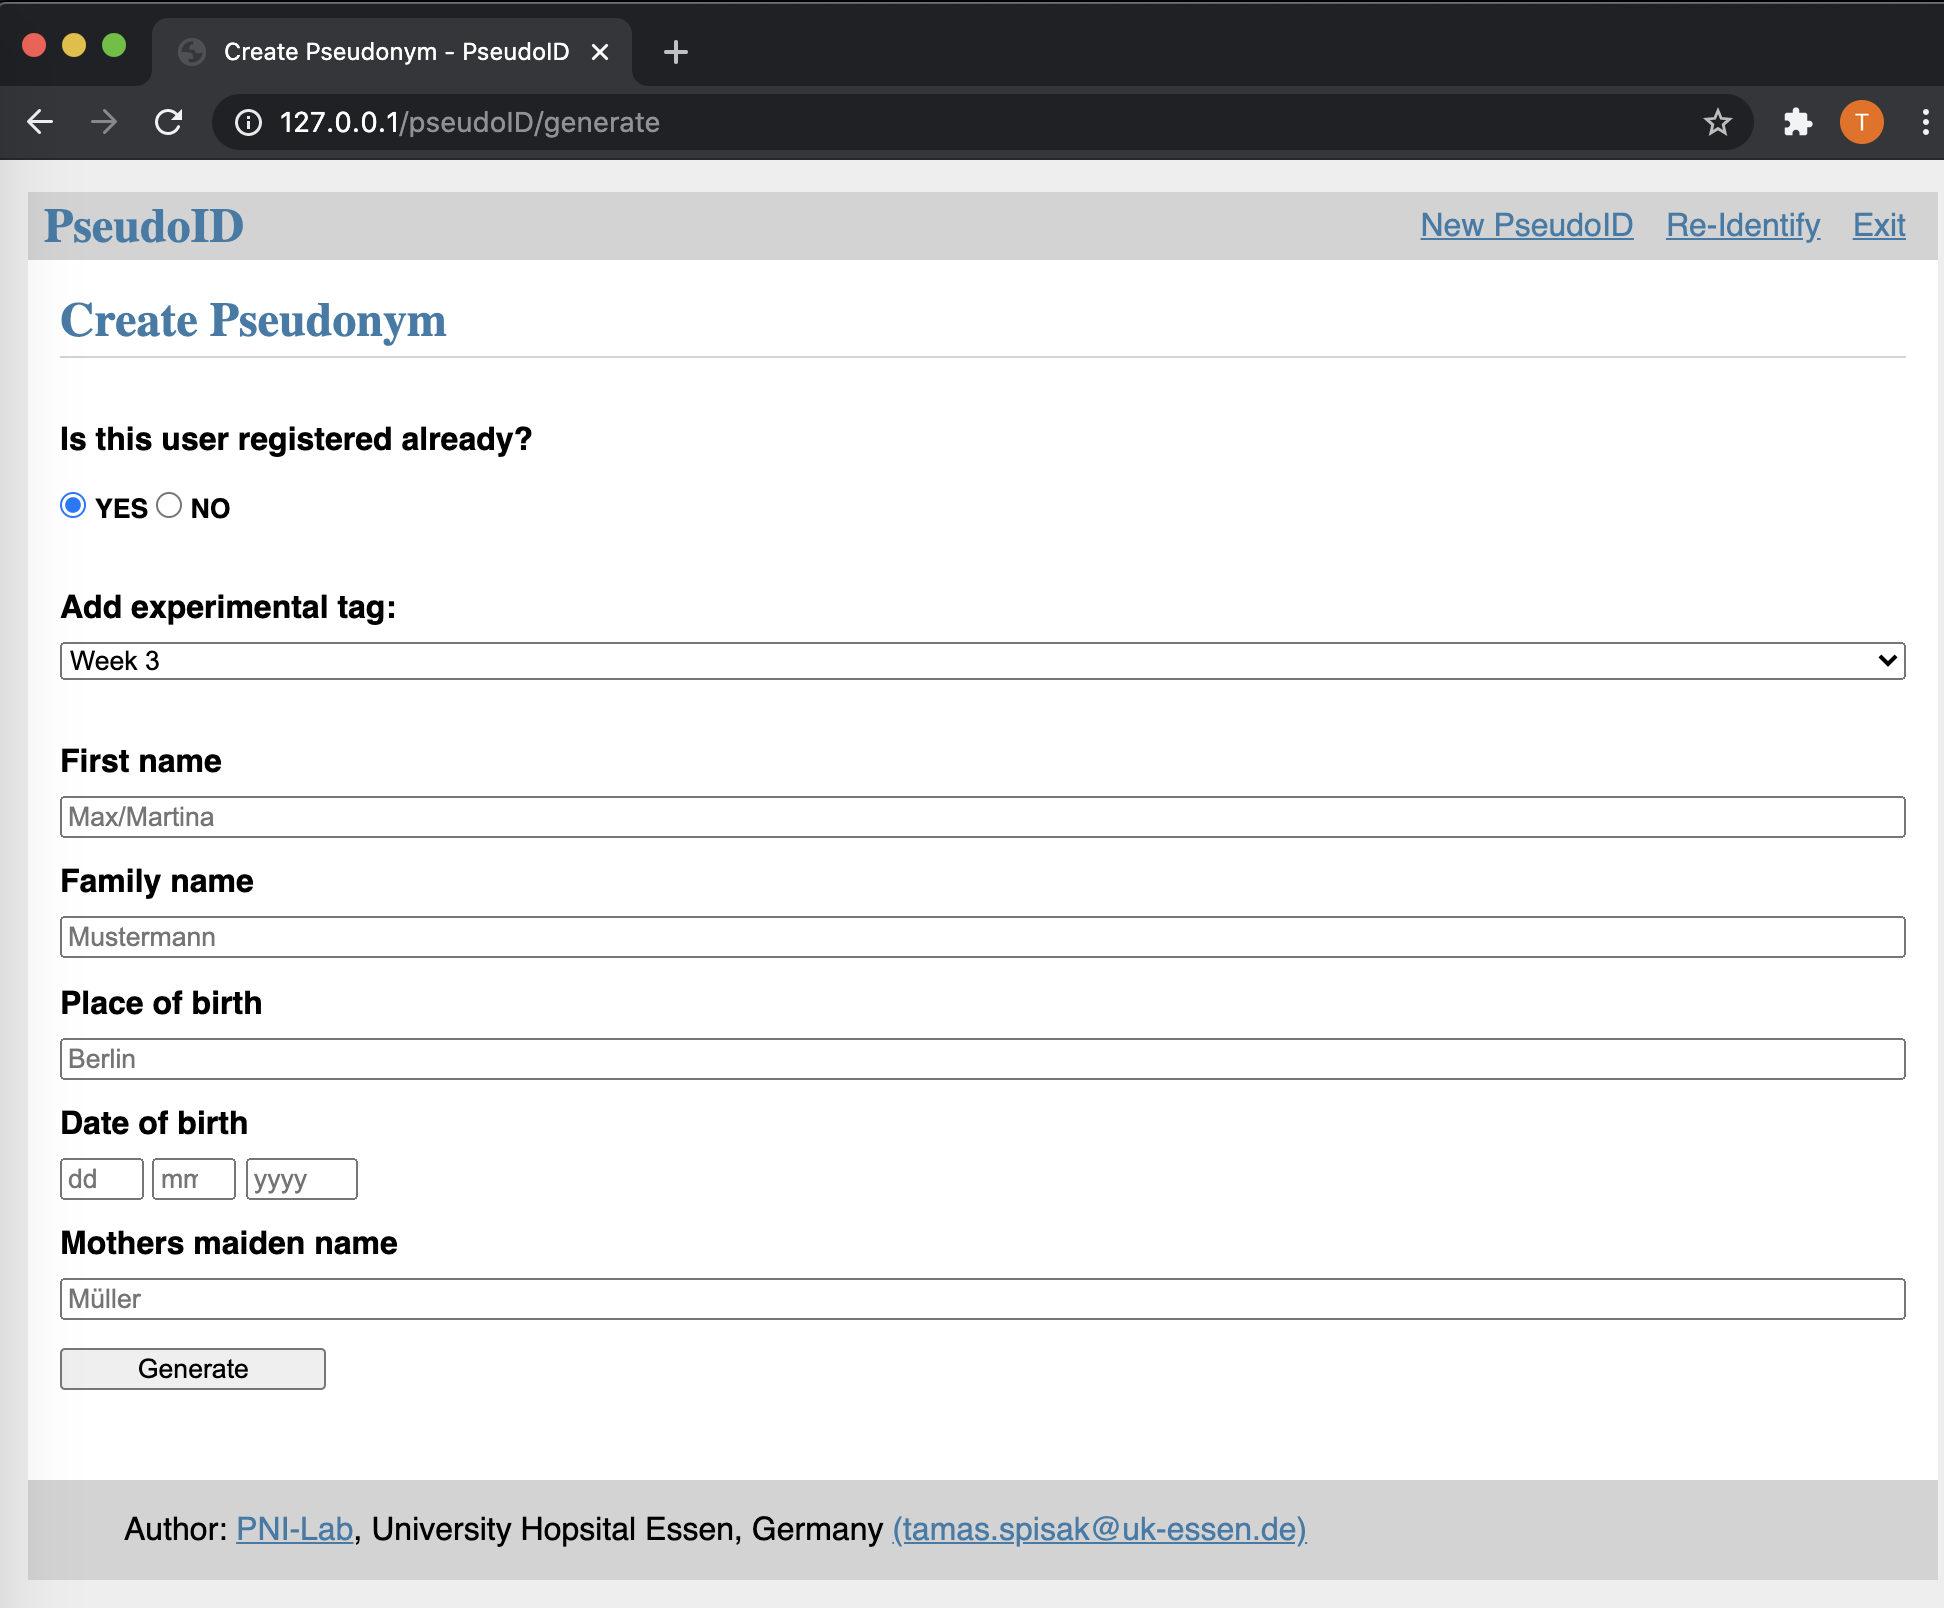
\includegraphics[width=.45\textwidth]{docs/fig/pseudoID_generate.png}}
\hfill
\subfigure{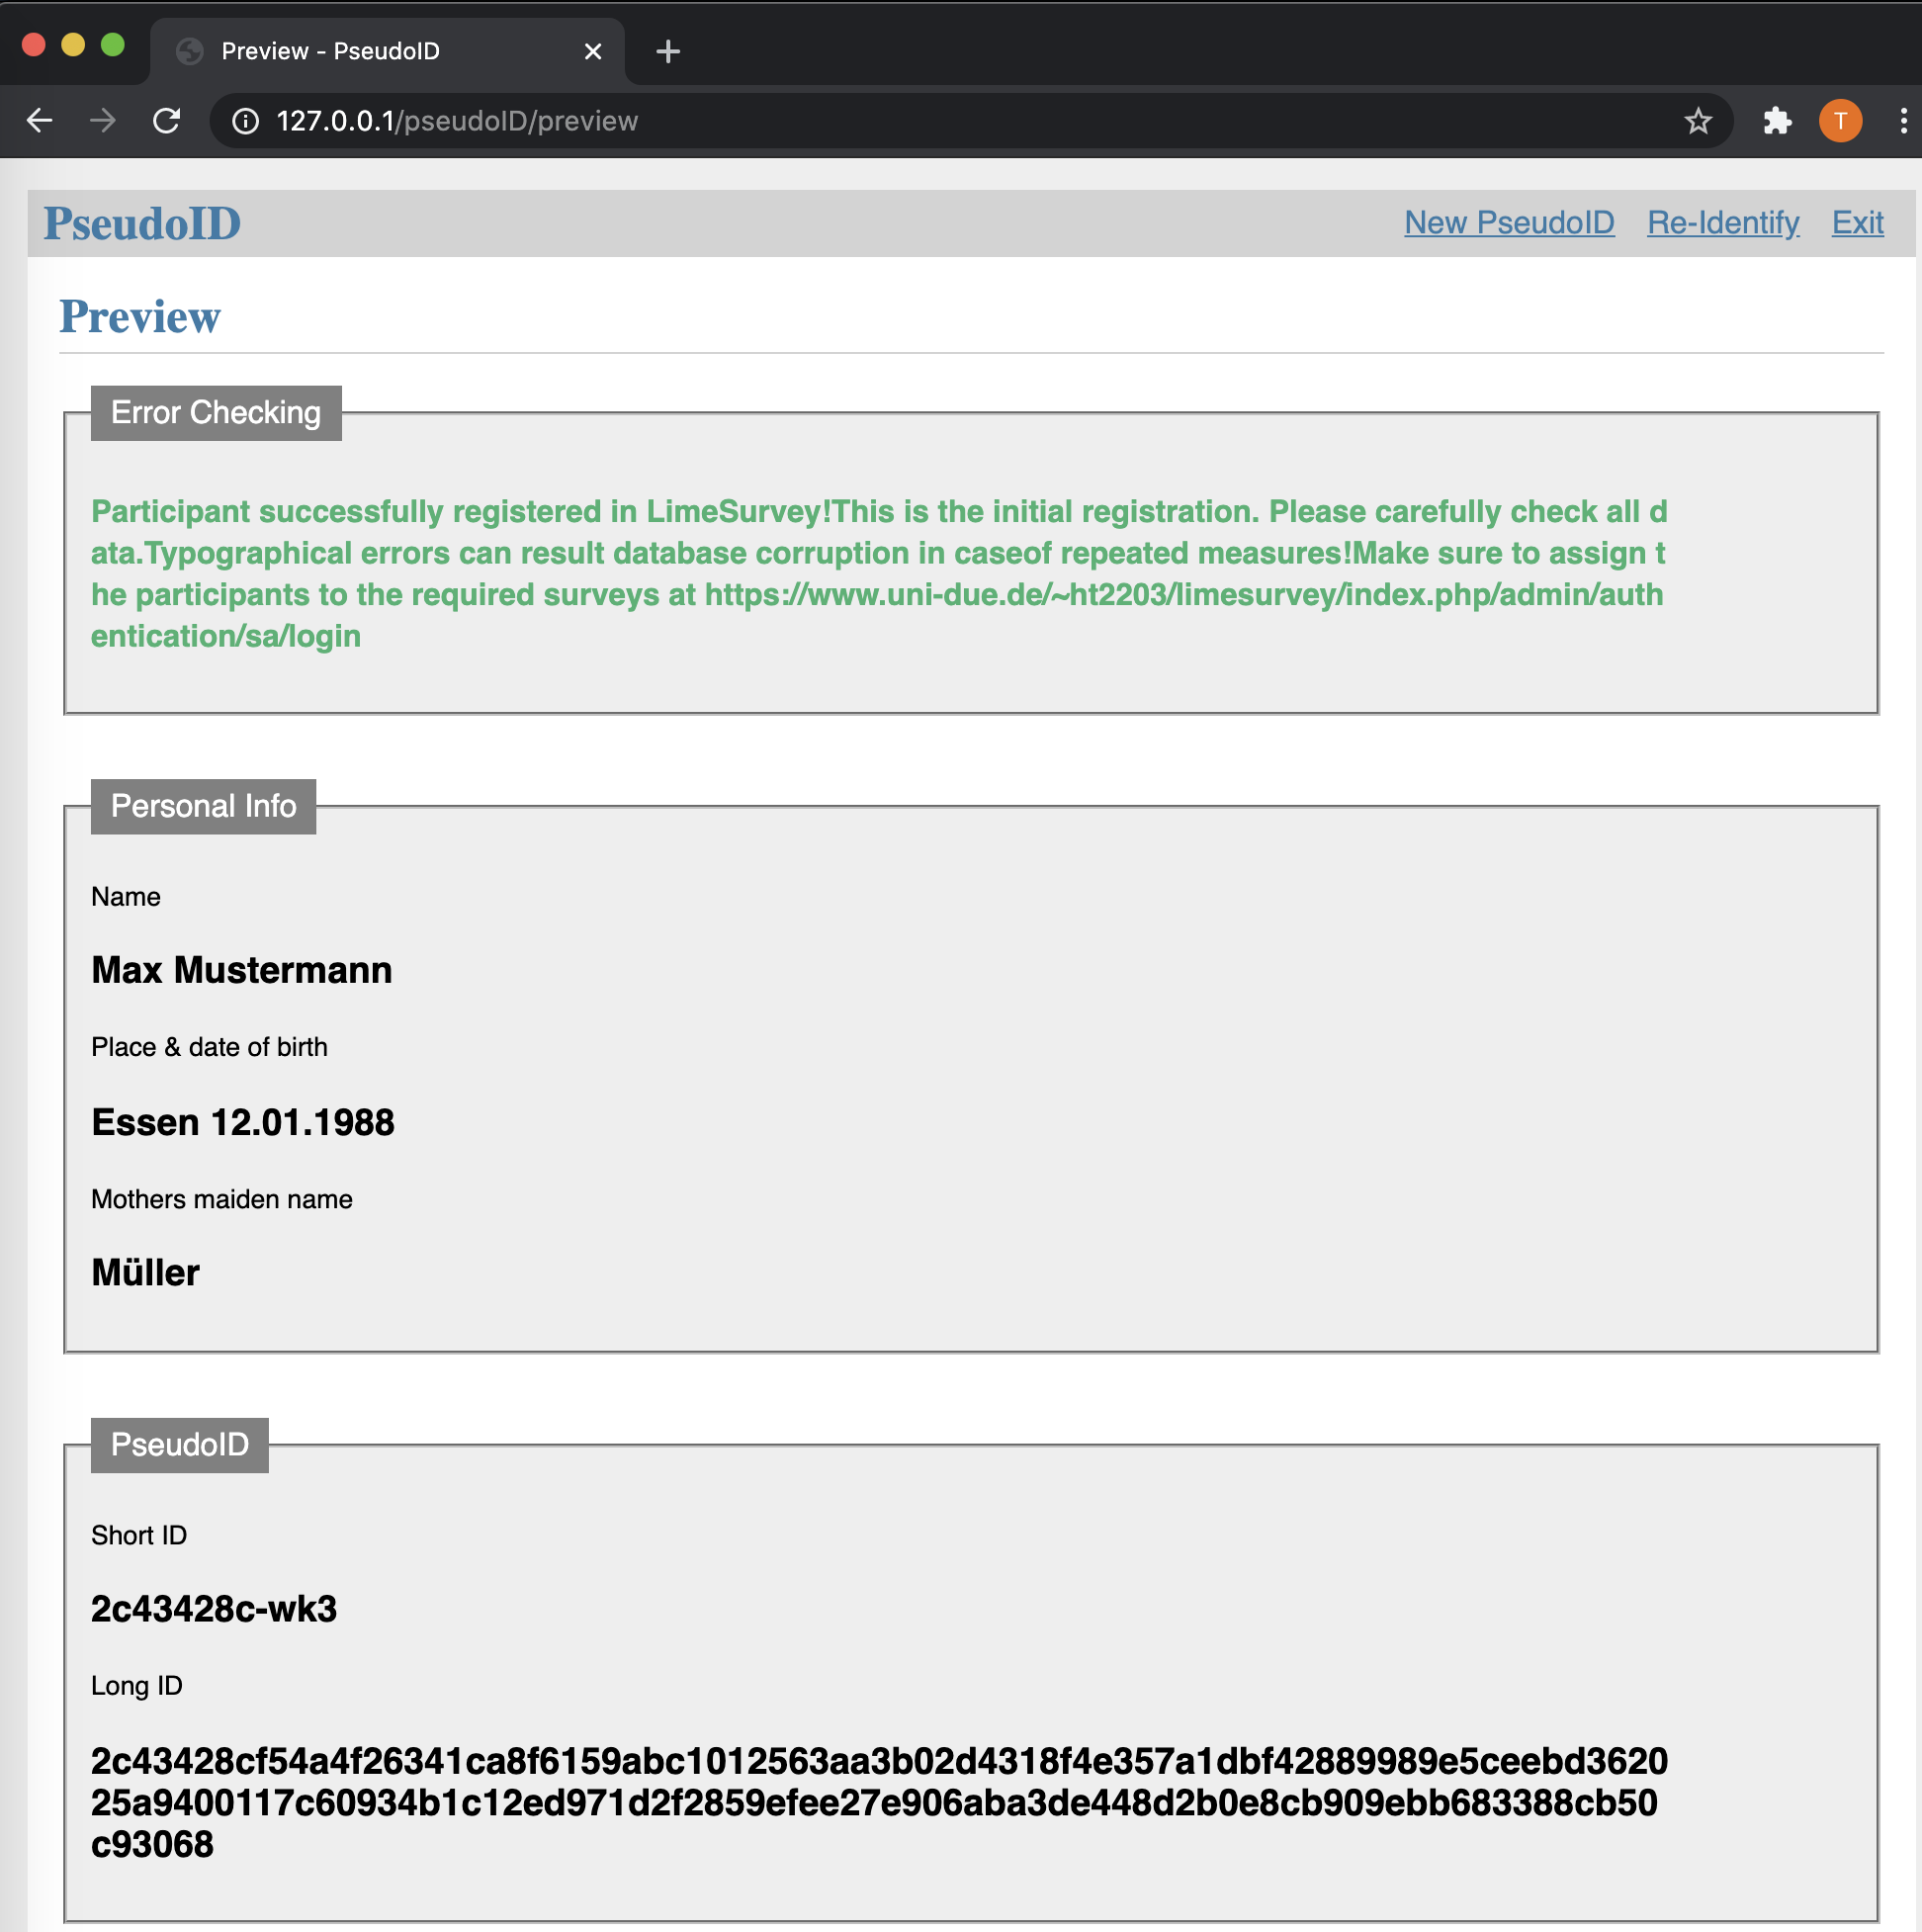
\includegraphics[width=.45\textwidth]{docs/fig/pseudoID_preview.png}}
\end{figure}

%\par\noindent\rule{\textwidth\color{pniblue}}{0.4pt}
\InsertBoxR{0}{
\small\setlength\fboxsep{5pt}\setlength\fboxrule{1pt}
\fcolorbox{pniblue}{pniblue!5}{\begin{minipage}{0.5\textwidth}
Importantly, even though the web browser is used as a user interface for the software (thus it looks like a webpage), personal data always stays on the local computer hosting the software and hardware key.
\end{minipage}}
}[1]
\lipsum[5]

